\documentclass[twocolumn]{article}

% Packages
\usepackage{graphicx}  % For including images
\usepackage{amsmath, amssymb}  % For math symbols
\usepackage{hyperref}  % For hyperlinks
\usepackage{geometry}  % Adjust page layout
\usepackage{titlesec}  % Section formatting
\usepackage{enumitem}  % for topsep, noitemsep
\usepackage{listings}  % for code environment
\usepackage{xcolor}

% packages table formatting
\usepackage{array}
\usepackage{longtable}
\usepackage{booktabs}

% graphics
\usepackage{pgfplots}
\usepackage{graphicx}
\pgfplotsset{compat=1.17}

% Define Python syntax highlighting
\lstdefinestyle{mystyle}{
    language=Python,
    basicstyle=\ttfamily\tiny,          % 8pt monospace
    keywordstyle=\bfseries,             % Bold keywords in blue
    commentstyle=\color{gray},          % Comments in gray
    stringstyle=\color{gray!80!black},  % Strings in red
    breaklines=true,                    % Allow line breaks
    frame=single,                       % Frame around the code
    captionpos=b                        % Caption at the bottom
}

% Define a common style for shell and PowerShell commands
\lstdefinestyle{shellstyle}{
    language=bash,                     % Use bash syntax (PowerShell is similar)
    basicstyle=\ttfamily\footnotesize,  % 8pt monospace
    keywordstyle=\bfseries,             % Bold commands
    commentstyle=\color{gray},          % Comments in gray
    stringstyle=\color{black},          % Strings in normal black
    backgroundcolor=\color{black!3},    % Light gray background
    frame=single,                        % Box around the command
    captionpos=b,                        % Caption at bottom
    breaklines=true                      % Allow line breaks
}

% Page Layout
\geometry{a4paper, margin=1in}

% Title Formatting
\titleformat{\section}{\Large\bfseries}{\thesection}{1em}{}

% Title Page
\title{
    %\includegraphics[width=0.3\textwidth]{logo.png} \\[1cm]
    \textbf{Progetto Rete Siamese} \\[0.5cm]
}
\author{Alessio Tanzi \\ Politecnico di Torino}
\date{\today}

\begin{document}

\maketitle

\begin{abstract}
    Questo documento dettaglia l'implementazione di una rete siamese. Lo scopo di questo progetto \`e l'implementazione di una rete neurale per il riconoscimento facciale tramite
    python, keras 2.10 (backend tensorflow 2.10).
\end{abstract}

\section{Teoria}
Una rete siamese usa \textit{Similarity} Learning*, ovvero cerca di imparare una funzione di similarit\`a 
tra due immagini.\par
Al fine di riconoscere una persona, le reti siamesi non prendono in input una singola immagine 
per ricondurla ad una delle "persone che la rete conosce" (essenzialmente una classe nota a priori), 
perch\`e costringerebbe un retraining ogni qual volta che si aggiunge una nuova persona 
da riconoscere, (e ti servono molte immagini per ogni persona).\par
La rete prende invece in input due immagini, 
\begin{itemize}[topsep=0pt, noitemsep]
    \item elabora ciascuna immagine attraverso due reti gemelle al fine di trasformare le immagini 
  in uno spazio delle features,
    \item utilizza una loss function comparativa per ottenere un indice di similarit\`a tra le due immagini
  e riconosci le due immagini come foto della stessa persona se tale misura \`e sufficientemente
  alta
\end{itemize}
L'architettura di tale rete si suddivide in due componenti fondamentali
\begin{itemize}[topsep=0pt, noitemsep]
    \item \textit{Embedding} Rete Convoluzionale che trasforma l'immagine nello spazio delle features. Se ne utilizzano una per ogni immagine processata in parallelo, dette \textit{Reti Gemelle}
    \item \textit{Calcolo della loss} Trasforma pi\`u immagini dallo spazio delle features in uno scalare rappresentante una misura di Costo
\end{itemize}
In particolare, in fase di Training, due possibili configurazioni
\begin{itemize}[topsep=0pt, noitemsep]
    \item \textit{Triplet Loss}: Utilizza tre reti gemelle per calcolare 3 embeddings, rispettivamente per 2 immagini simili, rappresentanti la stessa classe (\textit{Anchor} e \textit{Positive}),
        e una immagine differente (\textit{Negative}). Loss function:
        \[
            \mathcal{L}=\mathrm{max}\left(0, \mathrm{d}(a,p)-d(a,n)+m\right)
        \]
        Dove
        \begin{itemize}[topsep=0pt, noitemsep]
            \item[-] $d$: Funzione di distanza tra due embeddings, eg. norma L2 o \href{https://en.wikipedia.org/wiki/Cosine_similarity}{Cosine Similarity}\footnote{https://en.wikipedia.org/wiki/Cosine\_similarity}
            \item[-] $a$, $n$, $p$: Rispettivamente embeddings di Anchor, Negative, Positive
            \item[-] $m$: Margine settato a priori
        \end{itemize}
    \item \textit{Contrastive Loss}: In fase di training, si utilizza un dataset di coppie di immagini dotate di label. In particolare, sono presenti coppie di immagini labelled come "Simili" (1) e coppie
        "Dissimili" (0). Due reti gemelle calcolano calcolano in parallelo gli embeddings per le due immagini in input, e viene calcolata una funzione di Loss supervisionata:
        \[
            \mathcal{L}=\left(1-Y\right) \frac{1}{2}\left(D_W\right)^2 + (Y)\frac{1}{2}\left\{\mathrm{max}\left(0,m-D_W\right)\right\}^2
        \]
        Dove
        \begin{itemize}[topsep=0pt, noitemsep]
            \item[-] $D_W$ \`e la \textit{Distanza Euclidea} tra i due vettori $Y$ e $\hat{Y}$
            \item[-] $m$ \`e un \textit{margine} positivo, iperparametro che detta la distanza minima che i due vettori devono possedere per essere contati come diversi
            \item[-] $Y$ valore vero del label
        \end{itemize}
\end{itemize}

\section{Implementazione}
\subsection{Architettura}
La Rete Siamese implementata utilizza 3 reti gemelle di embedding, ciascune delle quali derivata dalla rete \textbf{Resnet50} con pesi preallenati da Imagenet, con gli ultimi layers fully connected rimossi
e sostituiti con 3 layers fully connected con ReLU e Batch Normalization, con un output nello spazio delle features con dimensionalit\`a $256$. Inoltre, tutti i pesi della Resnet preesistente, eccetto quelli
dell'ultimo layer convoluzionale sono congelati, al fine di preservare il pre-allenamento della rete (pratica di \textit{Transfer Learning}). \\
{\tiny (Riferimento Codice: \texttt{siamese\_first/siamese\_lib/layers.py:triplet\_embedding\_model})}.\par
In seguito alle reti di embedding parallele, viene calcolata la Triplet Loss sopracitata \\ {\tiny (Riferimento Codice: \texttt{siamese\_first/siamese\_lib/layers.py:DistanceLayer}) }.\par

\subsection{Dataset}
Il dataset di base \`e disponibile al \href{https://www.kaggle.com/datasets/alessiocorrado99/animals10}{seguente link}\footnote{https://www.kaggle.com/datasets/alessiocorrado99/animals10}. Tale dataset possiede
26000 immagini di animali suddivise in 10 categorie: dog, cat, horse, spyder, butterfly, chicken, sheep, cow, squirrel, elephant.\par
Tale dataset \`e stato rielaborato, raggruppando le immagini in triplette, delle quali, Anchor e Positive sono campionate dalla stessa categoria, mentre Negative \`e campionata da un'altra. \\
{\tiny (Riferimento Codice: \texttt{siamese\_second/\_\_main\_\_.py:ImageBag})}.\\
Il seguente frammento di codice rappresenta la preelaborazione effettuata su ogni immagine caricata
\begin{lstlisting}[style=mystyle, caption=Image Preprocessing]
def preprocess_image(file_path: tf.Tensor, target_size) -> tf.Tensor:
    if isinstance(file_path, (str, Path)):
        file_path = tf.convert_to_tensor(str(file_path), dtype=tf.string)
    img = tf.io.read_file(file_path)
    # capace di decodificare tutti i formati comuni tranne GIF
    img = tf.io.decode_jpeg(img, channels=3)
    # normalizzazione inclusa
    img = tf.image.convert_image_dtype(img, tf.float32)
    # 224 x 224 utilizzata di default
    img = tf.image.resize(img, target_size)
    return img
\end{lstlisting}

\section{Applicazione}
\subsection{Utilizzo}
Si assume che l'applicazione impacchettata sia stata scaricata dalle Releases \href{https://github.com/alexoz12v2/siameseNN}{GitHub}\footnote{https://github.com/alexoz12v2/siameseNN}, o, alternativamente, 
ottenuta da una build manuale seguendo la guida \texttt{README.md} ed effettuando
\begin{lstlisting}[style=shellstyle]
    bazel build //:app_zip.light
\end{lstlisting}
Il risultato ottenuto \`e un'applicazione da terminale, la quale va avviata dallo script \texttt{start.ps1} (Windows)/\texttt{start.sh} (Linux)
Esempio di sintassi Windows\footnote{Si assume che \texttt{powershell} sia stato avviato con \texttt{ExecutionPolicy=Bypass}}
\begin{lstlisting}[style=shellstyle]
    .\start.ps1 siamese_second -ArgumentList "--working-directory=$(Split-Path (Get-Location) -Parent)","--action=train"
\end{lstlisting}
Una volta avviata l'applicazione, essa
\begin{enumerate}[topsep=0pt, noitemsep]
    \item Carica le librerie dinamiche relative a CUDA e PyQt6
    \item Inizializza Tensorflow
    \item Effettua l'accesso su Kaggle e Scarica il dataset, se non esistente nella \texttt{working-directory} specificata
    \item Carica/Crea il dataset di triplette
    \item Carica/Crea il modello di rete neurale
\end{enumerate}
Una volta effettuati gli steps preliminari, l'applicazione entra in loop, in attesa della ricezione di uno dei seguenti comandi
\begin{table}[h]
    \centering
    \resizebox{\linewidth}{!}{%
    \begin{tabular}{>{\ttfamily}l p{0.7\linewidth}}
        \toprule
        \textbf{Command} & \textbf{Description} \\
        \midrule
        train <epochs: int> & Allena il modello con il numero di epoche specificate, serializzandone i pesi a fine epoca. (learning rate = $0.01$) \\
        \addlinespace[2pt]
        test & Valuta il modello sul dataset di testing. \\
        \addlinespace[2pt]
        \multicolumn{2}{>{\ttfamily}l}{visualize <dataset: train|val|test> <batch: int>} \\ & Mostra le prime 3 triplette del batch selezionato. \\
        \addlinespace[2pt]
        inference & Performa una predizione su una tripletta selezionata manualmente, riportando \textit{AP}, \textit{AN} e Cosine Similarities. \\
        \addlinespace[2pt]
        quit & Termina l'applicazione. \\
        \bottomrule
    \end{tabular}%
    }
    \caption{Lista comandi dell'applicazione}
\end{table}

\subsection{Risultati}
A seguito di 50 epoche di training, i seguenti sono i risultati ottenuti\footnotemark
\begin{table}[h]
    \centering
    \resizebox{\linewidth}{!}{%
    \begin{tabular}{l p{0.7\linewidth}}
        \toprule
        \textbf{Statistica} & \textbf{Risultato} \\
        \midrule
        Consumo RAM/Working Set & $9.5-15$ GB/$3.7-5$ GB \\
        GPU Memory & $2.7$ GB \\
        Elapsed Training Time & $7877$ s \\
        Training Time Per Epoch & $76$ s \\
        Train Loss/Validation Loss finale & $0.0259$/$0.0107$ \\
        Test Loss & $0.050804$ \\
        \bottomrule
    \end{tabular}%
    }
    \caption{Risultati}
\end{table}
\footnotetext{I risultati relativi al consumo risorse sono stati ottenuti su Windows 10, Mediante Sysinternals Process Explorer. Processore: Ryzen R7 3700x, 16 GB RAM, GPU: NVIDIA GTX 1070 8GB}

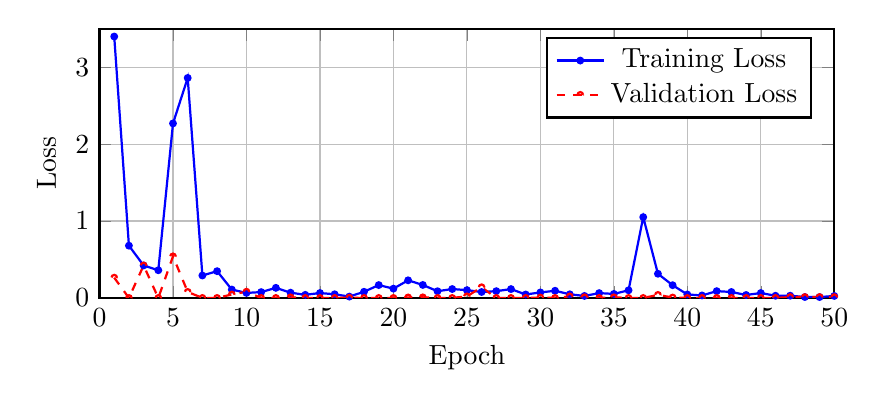
\begin{tikzpicture}
    \begin{axis}[
        width=0.9\linewidth,  % Fit within a two-column layout
        height=5cm,        % Adjust height as needed
        xlabel={Epoch},
        ylabel={Loss},
        legend pos=north east,
        grid=both,
        xmin=0, xmax=50,
        ymin=0, ymax=3.5,
        thick
    ]

    % Training Loss
    \addplot[color=blue, mark=*, mark size=1pt] 
    coordinates {
        (1, 3.3992) (2, 0.6797) (3, 0.4226) (4, 0.3602) (5, 2.2695) 
        (6, 2.8609) (7, 0.2918) (8, 0.3480) (9, 0.1091) (10, 0.0654)
        (11, 0.0762) (12, 0.1313) (13, 0.0685) (14, 0.0403) (15, 0.0640) 
        (16, 0.0478) (17, 0.0178) (18, 0.0802) (19, 0.1675) (20, 0.1210)
        (21, 0.2293) (22, 0.1690) (23, 0.0874) (24, 0.1159) (25, 0.1013) 
        (26, 0.0773) (27, 0.0883) (28, 0.1152) (29, 0.0448) (30, 0.0716)
        (31, 0.0933) (32, 0.0473) (33, 0.0261) (34, 0.0629) (35, 0.0524) 
        (36, 0.0995) (37, 1.0509) (38, 0.3143) (39, 0.1658) (40, 0.0453)
        (41, 0.0325) (42, 0.0885) (43, 0.0776) (44, 0.0385) (45, 0.0639) 
        (46, 0.0285) (47, 0.0293) (48, 0.0122) (49, 0.0115) (50, 0.0259)
    };
    \addlegendentry{Training Loss}

    % Validation Loss
    \addplot[color=red, mark=o, mark size=1pt, dashed] 
    coordinates {
        (1, 0.2639) (2, 0.0000) (3, 0.4226) (4, 0.0000) (5, 0.5408)
        (6, 0.0786) (7, 0.0000) (8, 0.0000) (9, 0.0452) (10, 0.0813)
        (11, 0.0000) (12, 0.0000) (13, 0.0082) (14, 0.0000) (15, 0.0000)
        (16, 0.0000) (17, 0.0029) (18, 0.0000) (19, 0.0000) (20, 0.0000)
        (21, 0.0068) (22, 0.0080) (23, 0.0000) (24, 0.0000) (25, 0.0210)
        (26, 0.1393) (27, 0.0000) (28, 0.0000) (29, 7.0529e-04) (30, 0.0053)
        (31, 0.0000) (32, 0.0200) (33, 0.0092) (34, 0.0000) (35, 0.0082)
        (36, 0.0000) (37, 0.0000) (38, 0.0395) (39, 0.0056) (40, 0.0000)
        (41, 0.0000) (42, 0.0000) (43, 0.0000) (44, 0.0000) (45, 3.9242e-04)
        (46, 0.0000) (47, 0.0117) (48, 0.0113) (49, 0.0114) (50, 0.0107)
    };
    \addlegendentry{Validation Loss}

    \end{axis}
\end{tikzpicture}
Dove le ultime due misure sono ottenute inserendo in input alla rete una tripletta per ogni categoria.
Di seguito i risultati delle inferenze:
\begin{figure*} % Span both columns
    \centering
    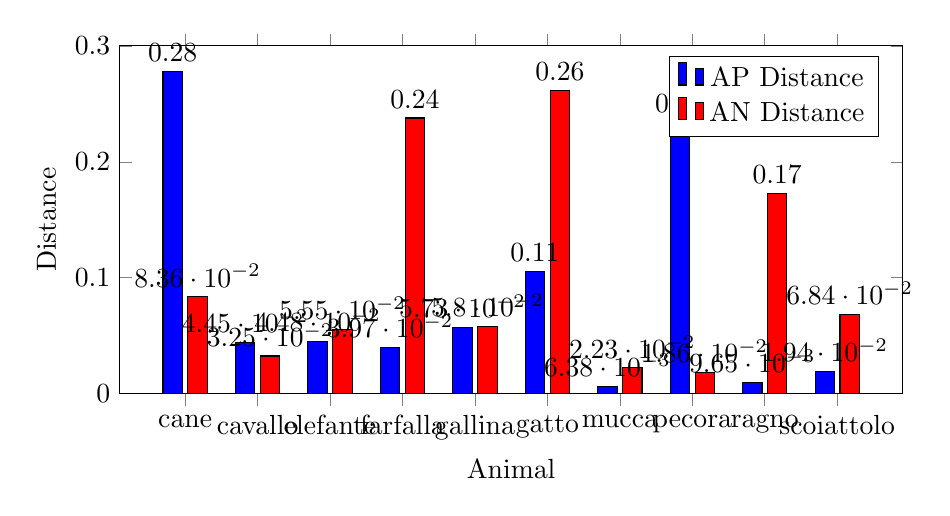
\begin{tikzpicture}
        \begin{axis}[
            width=0.95\textwidth, height=6cm,
            symbolic x coords={cane, cavallo, elefante, farfalla, gallina, gatto, mucca, pecora, ragno, scoiattolo},
            xtick=data,
            xlabel={Animal},
            ylabel={Distance},
            ybar,
            ymin=0, ymax=0.3,
            bar width=7pt,
            legend pos=north east,
            nodes near coords,
            enlarge x limits=0.1
        ]
        
        % AP Distance
        \addplot[fill=blue] coordinates {
            (cane, 0.277713) (cavallo, 0.044475) (elefante, 0.044843) (farfalla, 0.039670) 
            (gallina, 0.057287) (gatto, 0.105374) (mucca, 0.006384) (pecora, 0.234468) 
            (ragno, 0.009647) (scoiattolo, 0.019379)
        };
        \addlegendentry{AP Distance}

        % AN Distance
        \addplot[fill=red] coordinates {
            (cane, 0.083575) (cavallo, 0.032500) (elefante, 0.055507) (farfalla, 0.237782) 
            (gallina, 0.058021) (gatto, 0.261820) (mucca, 0.022331) (pecora, 0.018581) 
            (ragno, 0.172656) (scoiattolo, 0.068423)
        };
        \addlegendentry{AN Distance}
        
        \end{axis}
    \end{tikzpicture}
    \caption{AP and AN Distances for Different Animals}
    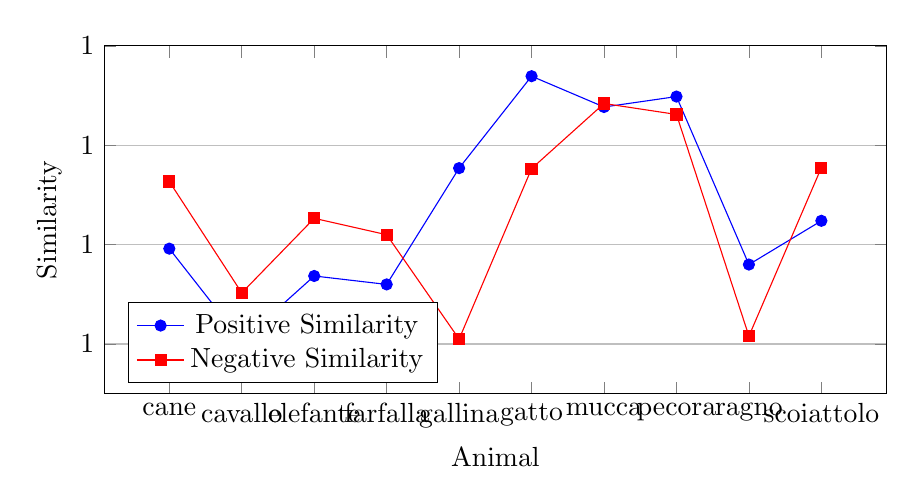
\begin{tikzpicture}
        \begin{axis}[
            width=0.95\textwidth, height=6cm,
            symbolic x coords={cane, cavallo, elefante, farfalla, gallina, gatto, mucca, pecora, ragno, scoiattolo},
            xtick=data,
            xlabel={Animal},
            ylabel={Similarity},
            ymin=0.9993, ymax=1.0000,
            ymajorgrids=true,
            mark size=2pt,
            legend pos=south west
        ]

        % Positive Similarity
        \addplot[mark=*, blue] coordinates {
            (cane, 0.999592) (cavallo, 0.999406) (elefante, 0.999537) (farfalla, 0.999520)
            (gallina, 0.999754) (gatto, 0.999939) (mucca, 0.999877) (pecora, 0.999898) 
            (ragno, 0.999560) (scoiattolo, 0.999648)
        };
        \addlegendentry{Positive Similarity}

        % Negative Similarity
        \addplot[mark=square*, red] coordinates {
            (cane, 0.999727) (cavallo, 0.999503) (elefante, 0.999653) (farfalla, 0.999620)
            (gallina, 0.999410) (gatto, 0.999753) (mucca, 0.999884) (pecora, 0.999862) 
            (ragno, 0.999416) (scoiattolo, 0.999755)
        };
        \addlegendentry{Negative Similarity}

        \end{axis}
    \end{tikzpicture}
    \caption{Positive and Negative Similarities for Different Animals}
    \resizebox{\linewidth}{!}{%
    \begin{tabular}{l p{0.7\linewidth}}
        \toprule
        \textbf{Statistica} & \textbf{Risultato} \\
        \midrule
        AP Distance/AN Distance & $	0.08334$/$	0.10183$ \\
        AP Cosine Similarity/AN Cosine Similarity & $0.999673$/$0.999659$ \\
        \bottomrule
    \end{tabular}%
    }
    \caption{Risultati}
\end{figure*}
\end{document}